\documentclass{article}
\usepackage[utf8]{inputenc}
\usepackage{graphicx}
\usepackage{hyperref}
\usepackage{geometry}
\geometry{a4paper} % Set the page size to A4
\usepackage{listings} % Package for including code in the document

\title{Práctica 07: Funciones en SQL}
\author{Carlos I. Padilla Herrera}
\date{13 de mayo de 2024}

\lstset{frame=single, % Adds a frame around the code
        basicstyle=\small\ttfamily, % Use a small, true type font
        language=SQL, % SQL syntax highlighting
        showstringspaces=false} % Don't mark spaces in strings

\begin{document}

\begin{titlepage}
    \centering
    \vspace*{1cm}
    \Huge\textbf{Curso de base de datos entre semana G0224}
    
    \vspace{0.5cm}
    \LARGE Escuela de Código PILARES
    
    \vspace{1.5cm}
    \textbf{Carlos Ignacio Padilla Herrera}
    
    \vspace{2cm}
    \Large\textbf{Folio:} 794DR02
    
    \vspace{0.5cm}
    \Large\textbf{Práctica 07:} Funciones en SQL.
    
    \vfill
    
    \Large\textbf{Fecha:} 13 de mayo de 2024.
    
    \vspace{0.8cm}
\end{titlepage}

\newpage

\section*{Código SQL para la creación de tablas y inserción de datos}

\begin{lstlisting}
-- Creating tables
create table manufacturer (
    code int(10) primary key,
    name varchar(100)
);

create table product (
    code int(10) primary key,
    name varchar(100),
    price double,
    manufacturer_code int(10),
    foreign key (manufacturer_code) references manufacturer(code)
);

-- Inserting manufacturers
insert into manufacturer (code, name) values
(1, 'Asus'),
(2, 'Lenovo'),
(3, 'Hewlett-Packard'),
(4, 'Samsung'),
(5, 'Seagate'),
(6, 'Crucial'),
(7, 'Gigabyte'),
(8, 'Huawei'),
(9, 'Xiaomi');

-- Inserting products
insert into product (code, name, price, manufacturer_code) values
(1, 'Disco Duro SATA3 1TB', 86.99, 5),
(2, 'Memoria RAM DDR4 8GB', 120, 6),
(3, 'Disco SSD 1TB', 150.99, 4),
(4, 'GeForce GTX 1050 Ti', 185, 7),
(5, 'GeForce GTX 1080 Xtreme', 755, 6),
(6, 'Monitor 24 LED Full HD', 202, 1),
(7, 'Monitor 27 LED Full HD', 245.99, 1),
(8, 'Portatil Yoga 520', 559, 2),
(9, 'Portatil Ideapad 320', 444, 2),
(10, 'Impresora HP Deskjet 3720', 59.99, 3),
(11, 'Impresora HP Laserjet Pro M26nw', 180, 3);
\end{lstlisting}

\newpage % Inicia una nueva página

\section*{1.Calcula el número total de productos que hay en la tabla productos.}


\begin{figure}[ht]
    \centering
    {
        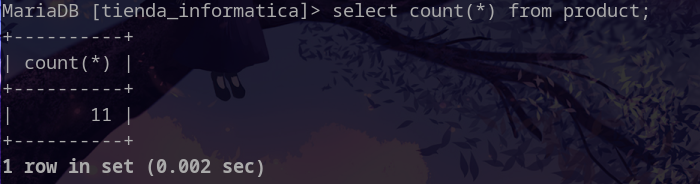
\includegraphics[width=\linewidth]{01screenshot.png} % Asegúrate de que el nombre del archivo y la extensión son correctos
    }
    \caption{Captura de pantalla del número total de productos de la tabla productos.}
\end{figure}

\newpage % Inicia una nueva página

\section*{2. Muestra el número total de productos que tiene cada uno de los fabricantes. 
El listado también debe incluir los fabricantes que no tienen ningún producto. 
El resultado mostrará dos columnas, una con el nombre del fabricante y otra con 
el número de productos que tiene. Ordene el resultado descendentemente por el número de productos.}

\begin{figure}[ht]
    \centering
    {
        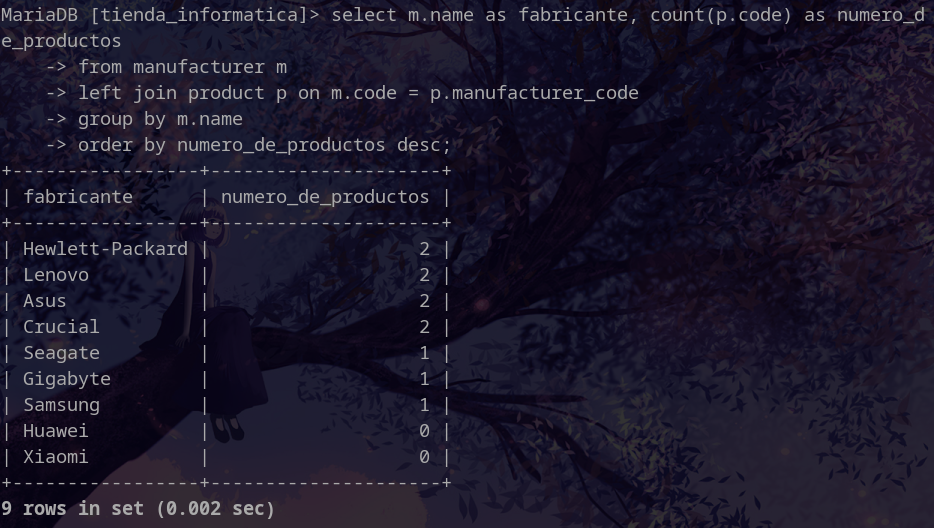
\includegraphics[width=\linewidth]{02screenshot.png} % Asegúrate de que el nombre del archivo y la extensión son correctos
    }
    \caption{Captura de pantalla del número total de productos de cada uno de los fabricantes.}
\end{figure}


\newpage % Inicia una nueva página

\section*{3. Muestra el precio máximo, precio mínimo y precio medio de los productos de cada uno de los fabricantes. 
El resultado mostrará el nombre del fabricante junto con los datos que se solicitan.}

\begin{figure}[ht]
    \centering
    {
        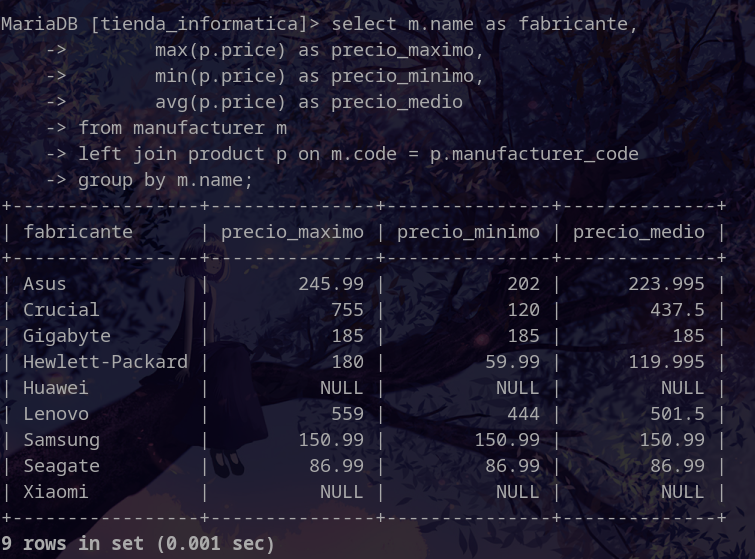
\includegraphics[width=\linewidth]{03screenshot.png} % Asegúrate de que el nombre del archivo y la extensión son correctos
    }
    \caption{Captura de pantalla del precio máximo, mínimo y medio de los productos de los fabricantes.}
\end{figure}
\newpage % Inicia una nueva página

\section*{4. Muestra el nombre de cada fabricante, junto con el precio máximo, 
precio mínimo, precio medio y el número total de productos de los fabricantes 
que tienen un precio medio superior a 200€. Es necesario mostrar el nombre del fabricante.}

\begin{figure}[ht]
    \centering
    {
        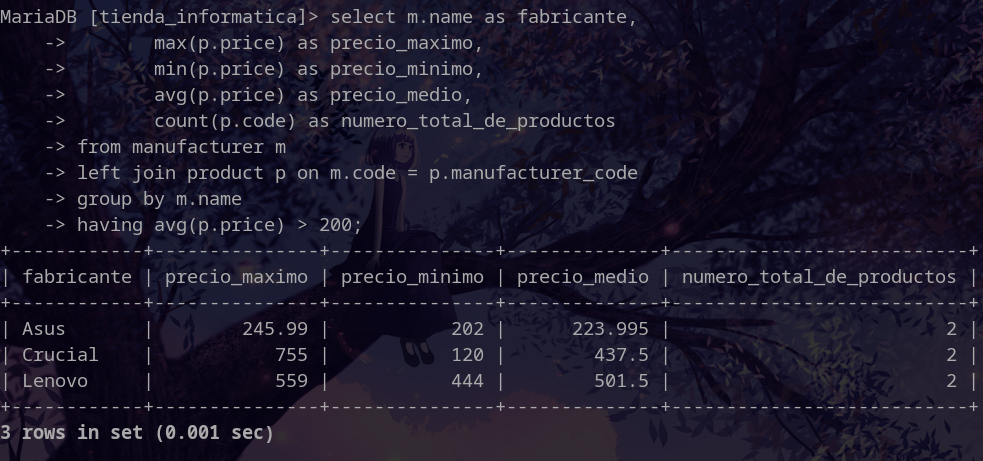
\includegraphics[width=\linewidth]{04screenshot.png} % Asegúrate de que el nombre del archivo y la extensión son correctos
    }
    \caption{Captura de pantalla del precio máximo, mínimo, medio y número total de productos con precio medio mayor a 200€
     de los productos de los fabricantes.}
\end{figure}

\end{document}
